% !TEX program = lualatex
% EC & BIOS 固件结构分析报告
% ThinkPad Z13 Gen1 (21D2) - EC SPI Flash Layout
\documentclass[a4paper,11pt,fontset=none]{ctexart}

% ── 字体 ──
\usepackage{fontspec}
\setmonofont{Menlo}[Scale=0.85]
\setCJKmainfont{Source Han Serif SC}[BoldFont={Source Han Serif SC SemiBold}]
\setCJKsansfont{Source Han Sans SC VF}[BoldFont={Source Han Sans SC VF}]
\setCJKmonofont{Source Han Sans SC VF}

% ── 颜色 ──
\usepackage[dvipsnames,svgnames,x11names,table]{xcolor}
\definecolor{eccolor}{HTML}{2E86C1}
\definecolor{pspcolor}{HTML}{E74C3C}
\definecolor{bioscolor}{HTML}{27AE60}
\definecolor{uefifv}{HTML}{8E44AD}
\definecolor{gapcolor}{HTML}{BDC3C7}
\definecolor{pdcolor}{HTML}{E67E22}
\definecolor{slotA}{HTML}{3498DB}
\definecolor{slotB}{HTML}{1ABC9C}

% ── 表格 ──
\usepackage{booktabs}
\usepackage{longtable}
\usepackage{multirow}
\usepackage{array}
\newcolumntype{R}[1]{>{\raggedleft\arraybackslash}p{#1}}
\newcolumntype{C}[1]{>{\centering\arraybackslash}p{#1}}

% ── 绘图 ──
\usepackage{tikz}
\usetikzlibrary{positioning, calc, fit, arrows.meta, decorations.pathreplacing, patterns}

% ── 字段图 ──
\usepackage{bytefield}

% ── 代码 ──
\usepackage{listings}
\lstset{
  basicstyle=\ttfamily\small,
  breaklines=true,
  frame=single,
  backgroundcolor=\color{gray!8},
  rulecolor=\color{gray!40},
  numbers=left,
  numberstyle=\tiny\color{gray},
  keywordstyle=\color{blue!70!black},
  commentstyle=\color{green!50!black},
}

% ── 超链接 ──
\usepackage[hidelinks,colorlinks=true,linkcolor=eccolor,urlcolor=pspcolor]{hyperref}

% ── 页面 ──
\usepackage[margin=2cm,headheight=14pt]{geometry}
\usepackage{fancyhdr}
\pagestyle{fancy}
\fancyhf{}
\fancyhead[L]{\small\textcolor{gray}{ThinkPad Z13 Gen1 固件分析}}
\fancyhead[R]{\small\textcolor{gray}{\thepage}}
\renewcommand{\headrulewidth}{0.4pt}

\usepackage{enumitem}

% ── 标题 ──
\title{\textbf{ThinkPad Z13 Gen1 EC \& BIOS 固件结构分析}\\[4pt]
  \large EC SPI Flash (W25Q256) 32MB 完整布局}
\author{逆向工程分析报告}
\date{2026-03-21}

\begin{document}
\maketitle
\tableofcontents
\clearpage

%% ════════════════════════════════════════════════════════════════════
\section{概览}

本文档对 ThinkPad Z13 Gen1 (型号 21D2) 的 EC SPI Flash 芯片 (Winbond W25Q256, 32MB) 进行完整的结构映射和固件版本变化分析。

\begin{itemize}[nosep]
  \item \textbf{主板}: NM-E161
  \item \textbf{EC SPI}: U8505, W25Q256JV, 32MB (256Mbit)
  \item \textbf{CPU}: AMD Rembrandt (Ryzen 6000)
  \item \textbf{EC MCU}: ARM Cortex-M 系列, Thumb-2 指令集
  \item \textbf{分析固件}: N3GHT25W v1.02 / N3GHT64W v1.64
\end{itemize}

%% ════════════════════════════════════════════════════════════════════
\section{SPI Flash 完整地图}

\subsection{32MB 全局视图}

\begin{center}
\begin{tikzpicture}[
  block/.style={draw, minimum width=13cm, minimum height=#1, anchor=north west,
    font=\small\ttfamily},
  label/.style={font=\small, anchor=east},
  scale=1
]

% 定义绘图参数 — 每 1MB = 0.45cm 高度
\def\mbtocm{0.45}
\def\totalh{14.4} % 32 * 0.45

% EC 区域 (0-1MB)
\node[block={\mbtocm cm}, fill=eccolor!25] (ec) at (0, 0)
  {EC 固件区域 — 双镜像 A/B + 管理数据};
\node[label] at (-0.2, 0) {\texttt{0x000000}};

% PSP 区域 (1-5MB)
\node[block={4*\mbtocm cm}, fill=pspcolor!20, below=0pt of ec.south west, anchor=north west] (psp)
  {AMD PSP 固件 — \$PL2 Directory + 46 组件};
\node[label] at (-0.2, {-\mbtocm}) {\texttt{0x100000}};

% BIOS L2 + APCB (5-5.3MB)
\node[block={0.3*\mbtocm cm}, fill=bioscolor!20, below=0pt of psp.south west, anchor=north west] (bios)
  {};
\node[label] at (-0.2, {-5*\mbtocm}) {\texttt{0x486000}};

% Secondary PSP/BIOS (5.3-7.5MB)
\node[block={2.2*\mbtocm cm}, fill=gapcolor!30, below=0pt of bios.south west, anchor=north west] (sec)
  {Secondary PSP / BIOS 备份};
\node[label] at (-0.2, {-5.3*\mbtocm}) {\texttt{0x4D7000}};

% UEFI FV (7.5-14.5MB)
\node[block={7*\mbtocm cm}, fill=uefifv!20, below=0pt of sec.south west, anchor=north west] (uefi)
  {UEFI Firmware Volume — 7168KB (\_FVH)};
\node[label] at (-0.2, {-7.5*\mbtocm}) {\texttt{0x787000}};

% Post-UEFI (14.5-16MB)
\node[block={1.5*\mbtocm cm}, fill=gapcolor!15, below=0pt of uefi.south west, anchor=north west] (post)
  {Post-UEFI + 空白至 16MB};
\node[label] at (-0.2, {-14.5*\mbtocm}) {\texttt{0xE87000}};

% Upper 16MB (16-32MB)
\node[block={2*\mbtocm cm}, fill=gapcolor!8, below=0pt of post.south west, anchor=north west] (upper)
  {上半 16MB — 大部分空白 (R1/R2 Journal)};
\node[label] at (-0.2, {-16*\mbtocm}) {\texttt{0x1000000}};

\node[label] at (-0.2, {-18*\mbtocm}) {\texttt{0x2000000}};

% 右侧大小标注
\draw[decorate, decoration={brace, amplitude=5pt, mirror}]
  (13.2, 0) -- (13.2, {-\mbtocm}) node[midway, right=6pt, font=\small] {1MB};
\draw[decorate, decoration={brace, amplitude=5pt, mirror}]
  (13.2, {-\mbtocm}) -- (13.2, {-5*\mbtocm}) node[midway, right=6pt, font=\small] {3.5MB};
\draw[decorate, decoration={brace, amplitude=5pt, mirror}]
  (13.2, {-7.5*\mbtocm}) -- (13.2, {-14.5*\mbtocm}) node[midway, right=6pt, font=\small] {7MB};

\end{tikzpicture}
\end{center}

\subsection{EC 区域详细视图 (0x000000 -- 0x100000)}

\begin{center}
\begin{tikzpicture}[
  block/.style={draw, minimum width=12cm, minimum height=#1, anchor=north west,
    font=\small\ttfamily},
  label/.style={font=\scriptsize\ttfamily, anchor=east},
]

\def\kbtocm{0.018}

% EC 管理数据
\node[block={4*\kbtocm cm}, fill=eccolor!10] (mgmt) at (0, 0)
  {EC 管理数据 (0x1000)};
\node[label] at (-0.2, 0) {0x000000};

% EC Image A
\node[block={316*\kbtocm cm}, fill=slotA!30, below=0pt of mgmt.south west, anchor=north west] (slotA)
  {\textcolor{slotA}{\textbf{EC Image A}} — N3GHT25W (316KB)};
\node[label] at (-0.2, {-4*\kbtocm}) {0x001000};

% Gap
\node[block={320*\kbtocm cm}, fill=gapcolor!20, below=0pt of slotA.south west, anchor=north west] (gap1)
  {中间数据 / 备用区域 (320KB)};
\node[label] at (-0.2, {-320*\kbtocm}) {0x050000};

% EC Image B
\node[block={316*\kbtocm cm}, fill=slotB!30, below=0pt of gap1.south west, anchor=north west] (slotB)
  {\textcolor{slotB}{\textbf{EC Image B}} — N3GHT22W (316KB, 旧版)};
\node[label] at (-0.2, {-640*\kbtocm}) {0x0A0000};

% EC tail
\node[block={68*\kbtocm cm}, fill=eccolor!10, below=0pt of slotB.south west, anchor=north west] (tail)
  {EC NV 存储 + 控制块};
\node[label] at (-0.2, {-956*\kbtocm}) {0x0EF000};

\node[label] at (-0.2, {-1024*\kbtocm}) {0x100000};

% 右侧标注
\draw[decorate, decoration={brace, amplitude=4pt, mirror}]
  (12.2, {-4*\kbtocm}) -- (12.2, {-320*\kbtocm})
  node[midway, right=5pt, font=\scriptsize] {316KB};
\draw[decorate, decoration={brace, amplitude=4pt, mirror}]
  (12.2, {-640*\kbtocm}) -- (12.2, {-956*\kbtocm})
  node[midway, right=5pt, font=\scriptsize] {316KB};

\end{tikzpicture}
\end{center}

%% ════════════════════════════════════════════════════════════════════
\section{EC 镜像内部结构}

\subsection{\_EC Header (256 bytes, ver=2)}

\begin{center}
\begin{bytefield}[bitwidth=1.4em, endianness=little]{32}
  \bitheader{0,7,8,15,16,23,24,31} \\
  \bitbox{8}{\texttt{\_}} & \bitbox{8}{\texttt{E}} & \bitbox{8}{\texttt{C}} & \bitbox{8}{\texttt{ver}} \\
  \bitbox{32}{flags (uint32)} \\
  \bitbox{32}{total\_size (uint32)} \\
  \bitbox{32}{data\_size (uint32)} \\
  \wordbox[lrt]{1}{保留字段 / 校验和}\\
  \skippedwords \\
  \wordbox[lrb]{1}{\scriptsize ...共 256 bytes}
\end{bytefield}
\end{center}

\begin{itemize}[nosep]
  \item \textbf{ver=1} (288 bytes): FL2 发布版格式, VT 偏移 +0x0120
  \item \textbf{ver=2} (256 bytes): 工程版格式, VT 偏移 +0x0100
\end{itemize}

\subsection{向量表 (80 entries, 320 bytes)}

\begin{longtable}{R{1.2cm} C{2cm} R{2.8cm} p{5cm}}
  \toprule
  \textbf{Index} & \textbf{类型} & \textbf{值 (N3GHT25W)} & \textbf{说明} \\
  \midrule
  \endhead
  0 & SP & \texttt{0x200C8000} & 初始栈指针 (SRAM 顶部) \\
  1 & Reset & \texttt{0x100701F5} & Reset handler (指向VT区数据) \\
  2 & NMI & \texttt{0x10070291} & NMI → CRT0 初始化区 \\
  3 & HardFault & \texttt{0x1007029D} & HardFault → CRT0 区 \\
  4--6 & MemMgmt..UsageFault & — & 系统异常 handler \\
  16 & IRQ0 & \texttt{0x100702FD} & \textbf{默认 handler} (19 个 IRQ 共用) \\
  19--79 & IRQ3--IRQ63 & \texttt{0x1008xxxx} & 活跃 IRQ handler (37 个唯一) \\
  \bottomrule
\end{longtable}

\subsection{启动流程}

\begin{center}
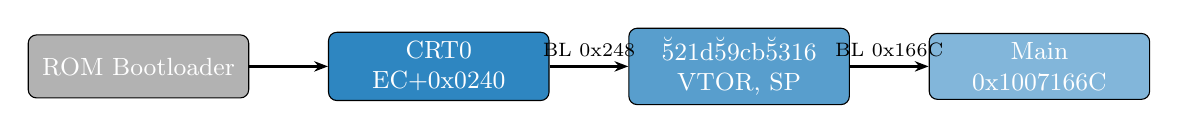
\begin{tikzpicture}[
  box/.style={draw, rounded corners=3pt, fill=#1, minimum width=2.8cm, minimum height=0.8cm, 
    font=\small, text=white, align=center},
  arr/.style={-{Stealth[length=5pt]}, thick},
]
  \node[box=gray!60] (rom) {ROM Bootloader};
  \node[box=eccolor, right=1cm of rom] (crt0) {CRT0\\EC+0x0240};
  \node[box=eccolor!80, right=1cm of crt0] (init) {\u521d\u59cb\u5316\\VTOR, SP};
  \node[box=eccolor!60, right=1cm of init] (main) {Main\\0x1007166C};
  
  \draw[arr] (rom) -- (crt0);
  \draw[arr] (crt0) -- (init) node[midway, above, font=\scriptsize] {BL 0x248};
  \draw[arr] (init) -- (main) node[midway, above, font=\scriptsize] {BL 0x166C};
\end{tikzpicture}
\end{center}

\subsection{内存映射}

\begin{longtable}{R{3cm} R{3cm} R{2cm} p{4cm}}
  \toprule
  \textbf{起始地址} & \textbf{结束地址} & \textbf{大小} & \textbf{用途} \\
  \midrule
  \endhead
  \texttt{0x10070000} & \texttt{0x100BF000} & 316KB & EC Flash (代码+数据) \\
  \texttt{0x200C0000} & \texttt{0x200C8000} & 32KB & SRAM \\
  \texttt{0x40000000} & \texttt{0x4F672004} & — & 外设寄存器 \\
  \texttt{0xE000ED08} & — & — & SCB\_VTOR \\
  \texttt{0xE000E100} & — & — & NVIC\_ISER0 \\
  \bottomrule
\end{longtable}

%% ════════════════════════════════════════════════════════════════════
\section{EC 固件版本演化}

\subsection{跨版本对比表}

\begin{longtable}{l C{1cm} R{1.2cm} R{2.5cm} R{2.5cm} R{1.8cm}}
  \toprule
  \textbf{版本} & \textbf{\_EC} & \textbf{Size} & \textbf{Base} & \textbf{SP} & \textbf{VT 偏移} \\
  \midrule
  \endhead
  N3GHT05T & v2 & 224K & \texttt{0x10070000} & \texttt{0x200C8000} & +0x0100 \\
  N3GHT07T & v2 & 224K & \texttt{0x10070000} & \texttt{0x200C8000} & +0x0100 \\
  N3GHT08M & v2 & 224K & \texttt{0x10070000} & \texttt{0x200C8000} & +0x0100 \\
  N3GHT11M & v2 & 320K & \texttt{0x10070000} & \texttt{0x200C8000} & +0x0100 \\
  N3GHT12W & v2 & 320K & \texttt{0x10070000} & \texttt{0x200C8000} & +0x0100 \\
  N3GHT14T & v2 & 320K & \texttt{0x10070000} & \texttt{0x200C8000} & +0x0100 \\
  N3GHT15W & v2 & 320K & \texttt{0x10070000} & \texttt{0x200C8000} & +0x0100 \\
  N3GHT22W & v2 & 316K & \texttt{0x10070000} & \texttt{0x200C8000} & +0x0100 \\
  N3GHT25W & v2 & 316K & \texttt{0x10070000} & \texttt{0x200C8000} & +0x0100 \\
  \rowcolor{yellow!15}
  N3GHT64W & v2 & 316K & \texttt{0x10070000} & \texttt{0x200C7C00} & +0x0100 \\
  \rowcolor{yellow!15}
  N3GHT68W & v1 & 320K & \texttt{0x10070000} & \texttt{0x200C7C00} & +0x0120 \\
  \rowcolor{yellow!15}
  N3GHT69W & v1 & 320K & \texttt{0x10070000} & \texttt{0x200C7C00} & +0x0120 \\
  \bottomrule
\end{longtable}

\noindent\textbf{关键变化}（黄色行）：
\begin{itemize}[nosep]
  \item N3GHT64W 起 SP 从 \texttt{0x200C8000} 降至 \texttt{0x200C7C00}（减少 1KB）
  \item N3GHT68W/69W 改用 FL2 发布格式（ver=1, VT 偏移 +0x0120）
\end{itemize}

\subsection{镜像大小演化}

\begin{center}
\begin{tikzpicture}[scale=0.9]
  \draw[->] (0,0) -- (13,0) node[right] {版本};
  \draw[->] (0,0) -- (0,5) node[above] {大小 (KB)};
  
  % 网格
  \foreach \y in {1,...,4} {
    \draw[gray!20] (0,\y) -- (13,\y);
  }
  \draw[gray!20] (0,3.2) -- (13,3.2); % 320K
  \draw[gray!20] (0,3.16) -- (13,3.16); % 316K
  
  % Y轴标签
  \node[left, font=\scriptsize] at (0,2.24) {224K};
  \node[left, font=\scriptsize] at (0,3.16) {316K};
  \node[left, font=\scriptsize] at (0,3.2) {320K};
  
  % 数据点
  \foreach \x/\v/\s in {
    1/05T/2.24, 2/07T/2.24, 3/08M/2.24,
    4/11M/3.2, 5/12W/3.2, 6/14T/3.2, 7/15W/3.2,
    8/22W/3.16, 9/25W/3.16, 10/64W/3.16,
    11/68W/3.2, 12/69W/3.2
  } {
    \fill[eccolor] (\x, \s) circle (3pt);
    \node[below, font=\tiny, rotate=45, anchor=north east] at (\x, 0) {\v};
  }
  
  % 连线
  \draw[eccolor, thick] (1,2.24) -- (2,2.24) -- (3,2.24) -- (4,3.2) -- (5,3.2) -- (6,3.2) -- (7,3.2) -- (8,3.16) -- (9,3.16) -- (10,3.16) -- (11,3.2) -- (12,3.2);
  
\end{tikzpicture}
\end{center}

\subsection{EC A/B 双镜像机制}

大型 SPI dump (N3GHT25W, N3GHT64W) 中发现 EC 采用 A/B 交替更新:

\begin{center}
\begin{tabular}{l l l l}
  \toprule
  \textbf{Dump} & \textbf{Slot A (0x001000)} & \textbf{Slot B (0x0A0000)} & \textbf{说明} \\
  \midrule
  N3GHT25W\_v1.02 & \textcolor{slotA}{N3GHT25W} & \textcolor{slotB}{N3GHT22W} & B 保留上一版本 \\
  N3GHT64W\_v1.64 & \textcolor{slotA}{N3GHT64W} & \textcolor{slotB}{N3GHT64W} & A/B 相同版本 \\
  早期工程版 & 仅 Slot A & (空) & 单镜像 \\
  \bottomrule
\end{tabular}
\end{center}

%% ════════════════════════════════════════════════════════════════════
\section{PSP 固件组件}

AMD PSP (Platform Security Processor) 固件位于 SPI 0x106000, 由 \texttt{\$PL2} 目录索引。

\subsection{PSP L2 组件清单}

\begin{longtable}{R{1cm} p{3.5cm} R{1.5cm} R{2.5cm} p{3cm}}
  \toprule
  \textbf{Type} & \textbf{名称} & \textbf{大小} & \textbf{SPI 偏移} & \textbf{说明} \\
  \midrule
  \endhead
  0x00 & AMD\_PUBLIC\_KEY & 1KB & 0x106400 & AMD 签名公钥 \\
  0x01 & PSP\_BL & 7KB & 0x106900 & PSP 启动加载器 \\
  0x73 & TPM\_SPI & 75KB & 0x108700 & fTPM 固件 \\
  0x02 & PSP\_TRUSTED\_OS & 89KB & 0x11AF00 & PSP 可信 OS \\
  0x08 & SMU\_FW & 135KB ×2 & 0x131400 & 系统管理单元 \\
  0x0C & BOOT\_TRUSTLETS & 136KB & 0x175200 & 信任链 \\
  0x24 & MP2\_FW & 19KB & 0x1D8000 & 传感器集线器 \\
  0x25 & DRIVER\_ENTRIES & 176KB & 0x1DCE00 & PSP 驱 \\
  0x30 & ABL0 & 459KB & 0x22D900 & AMD Boot Loader \\
  0x44 & DIAG\_BL & 67KB ×2 & 0x2A1800 & 诊断启动 \\
  \rowcolor{pdcolor!10}
  0x5A & USB4\_DXIO\_PHY & 308KB & 0x2CA800 & USB4 PHY 固件 \\
  0x5F & DXIO\_PHY\_FW & 384KB & 0x326000 & DXIO PHY 固件 \\
  0x47 & PSP\_SEV & 16KB & 0x2C2A00 & 安全加密虚拟化 \\
  0x49 & BIOS\_L2\_DIR & 1KB & 0x486000 & BIOS 组件目录 \\
  \bottomrule
\end{longtable}

\subsection{跨版本固件匹配率}

首 64KB 字节级对比 (N3GHT25W vs N3GHT64W):

\begin{center}
\begin{tikzpicture}[scale=0.8]
  \def\barw{0.6}
  \foreach \i/\name/\pct/\col in {
    1/AMD TA/81.7/bioscolor,
    2/MP2 Data/92.4/bioscolor,
    3/PSP BL/3.3/pspcolor,
    4/TPS PD/29.0/pdcolor,
    5/UEFI FV/0.7/pspcolor,
    6/APOB/47.6/gapcolor%
  } {
    \fill[\col!60] (\i*1.8-\barw/2, 0) rectangle (\i*1.8+\barw/2, \pct*0.04);
    \node[above, font=\scriptsize] at (\i*1.8, \pct*0.04) {\pct\%};
    \node[below, font=\scriptsize, rotate=30, anchor=north east] at (\i*1.8, 0) {\name};
  }
  \draw[->] (0,0) -- (12,0);
  \draw[->] (0,0) -- (0,4.5) node[above, font=\scriptsize] {匹配率};
\end{tikzpicture}
\end{center}

%% ════════════════════════════════════════════════════════════════════
\section{BIOS 与 UEFI 组件}

\subsection{BIOS L2 目录 (\$BL2)}

\begin{tabular}{R{1cm} p{5cm} R{2cm} R{3cm}}
  \toprule
  \textbf{Type} & \textbf{名称} & \textbf{大小} & \textbf{SPI 偏移} \\
  \midrule
  0x60 & APCB\_DATA & 12KB & 0x107000 \\
  0x68 & BIOS\_PSP\_PROVISION & 12KB & 0x116000 \\
  0x62 & BIOS\_RTM\_VOLUME & 1.75MB & 0x1F40000 \\
  0x64 & BIOS\_RTM\_SIGNATURE & 25KB & 0x141000 \\
  0x66 & BIOS\_COPY\_2 & 6KB ×2 & 0x14D900 \\
  \bottomrule
\end{tabular}

\subsection{UEFI Firmware Volume}

\begin{itemize}[nosep]
  \item \textbf{位置}: SPI 0x787000
  \item \textbf{大小}: 7168KB (7MB)
  \item \textbf{\_FVH 标志}: SPI 0x787028
  \item \textbf{FV GUID}: \texttt{5473c07a-3dcb-4dca-bd6f-1e9689e7349a}
  \item \textbf{熵}: 7.94 bits/byte (高度压缩)
\end{itemize}

%% ════════════════════════════════════════════════════════════════════
\section{IRQ Handler 分析}

\subsection{向量表使用情况}

80 个向量表条目中:
\begin{itemize}[nosep]
  \item \textbf{56 个唯一 handler 地址} (每版本)
  \item \textbf{19 个 IRQ} 共用默认 handler (EC+0x02FC)
  \item \textbf{37 个活跃 IRQ} handler, 代码位于 EC+0x1xxxx 区域
  \item \textbf{全部 74 个 handler} 在不同版本间均有变化
  \item \textbf{12 个唯一版本签名} — 每个版本的 handler profile 都不同
\end{itemize}

\subsection{Handler 变体分组}

\begin{center}
\begin{tabular}{l l}
  \toprule
  \textbf{变体数} & \textbf{Handler 类型} \\
  \midrule
  4 & 默认 handler (主要变化) \\
  11--12 & 大部分活跃 IRQ handler (几乎每版本不同) \\
  \bottomrule
\end{tabular}
\end{center}

%% ════════════════════════════════════════════════════════════════════
\section{LADD 描述符}

SPI dump 中存在 3 个 LADD (Load Address Descriptor) 结构:

\begin{enumerate}[nosep]
  \item \textbf{EC 内部 LADD} @ SPI 0x044FE2 — EC 固件模块分发表,包含 EUER, EDER, EWEB, EREB 等模块入口
  \item \textbf{EC 内部 LADD (副本)} @ SPI 0x0E2E3A — 位于 PSP 固件区域 (属于另一个固件上下文)
  \item \textbf{Flash 主目录} @ SPI 0x100000 — 整个 SPI 的区域映射, 26 个条目
\end{enumerate}

Flash 主 LADD 格式: \texttt{LADDR\textbackslash{}x00} + 条目对 (SPI\_offset, size), 以 \texttt{0xFFFFFFFF} 结尾。

%% ════════════════════════════════════════════════════════════════════
\section{TPS PD 控制器固件}

SPI 0x2C1000 区域 (676KB) 包含 TI TPS65988 USB-C PD 控制器固件:

\begin{itemize}[nosep]
  \item 包含 2 个 \textbf{TPSHTRMP} 标签 (TPS Host Trampoline)
  \item 低熵 (0.56 bits/byte, 大量 0x00 填充), 实际代码集中在后半部分
  \item 跨版本匹配率 29\% — PD 固件有显著更新
  \item PSP 通过 type=0x5A 条目引用 USB4 DXIO PHY 固件 (308KB)
\end{itemize}

%% ════════════════════════════════════════════════════════════════════
\section{工具脚本清单}

\begin{longtable}{p{5cm} p{8cm}}
  \toprule
  \textbf{脚本} & \textbf{功能} \\
  \midrule
  \endhead
  \texttt{ec\_extract\_blob.py} & 从 SPI dump 提取 EC blob \\
  \texttt{ghidra\_ec\_loader.py} & Ghidra 加载脚本 (VT, 内存映射, 符号) \\
  \texttt{ida\_ec\_loader.py} & IDA Pro 加载脚本 \\
  \texttt{ec\_cross\_base\_analysis.py} & 跨版本基地址/VT/启动流分析 \\
  \texttt{ec\_irq\_compare.py} & IRQ handler 签名对比 \\
  \texttt{ec\_large\_regions.py} & SPI 大型区域扫描 \\
  \texttt{ec\_ladd\_psp\_parse.py} & LADD 目录 + PSP \$PL2 解析 \\
  \texttt{ec\_ab\_layout.py} & EC A/B 双镜像布局检测 \\
  \texttt{ec\_ldr\_scan.py} & LDR 指令基地址扫描器 \\
  \texttt{ec\_base\_verify.py} & 基地址验证 (flash/SRAM/peripheral refs) \\
  \bottomrule
\end{longtable}

\end{document}
